\newpage
\thispagestyle{empty}

%\markboth{ \mbox{M\'{E}TODO  DA M\'{A}XIMA VEROSSIMILHAN\c{C}A} }{ \mbox{ESTIMADORES DE M\'{A}XIMA VEROSSIMILHAN\c{C}A} }

\noindent {\huge \bf 5 }

\vspace{1cm}
%\hspace*{-0.5cm} {\huge \bf M\'{e}todo~da~m\'{a}xima~verossimilhan\c{c}a} \index{metodo@m\'{e}todo! da m\'{a}xima verossimilhan\c{c}a}\index{maxima@m\'{a}xima verossimilhan\c{c}a! m\'{e}todo da}
\hspace*{-0.5cm} {\huge \bf Determina\c{c}\~{a}o de par\^{a}metros} \index{determina\c{c}\~{a}o de par\^{a}metros}\index{par\^{a}metros! determina\c{c}\~{a}o de}

%\addcontentsline{toc}{chapter}{5 \quad M\'{e}todo da m\'{a}xima verossimilhan\c{c}a}
\addcontentsline{toc}{chapter}{5 \quad Determina\c{c}\~{a}o de par\^{a}metros}
%ve\-ros\-si\-mi\-lhan\-\c{c}a

\setcounter{chapter}{5}
\setcounter{section}{0}
\setcounter{figure}{0}
\setcounter{table}{0}
\setcounter{equation}{0}
\label{Likeli}
%\newpage
%\thispagestyle{empty}

% \chapter{Estimativas de par\^{a}metros} \index{estimativas! de par\^{a}metros}
% \index{par\^{a}metros! estimativas de}
%\label{Erros}


%\def\figurename{\small Fig.~\ref{Erros}.}
%\def\tablename{\small Tab.~\ref{Erros}.}
%\newpage
%\ \\


\begin{flushright}
\begin{minipage}{8cm}
{\small
\baselineskip=8.5pt
{\it   Os problemas de estima\c{c}\~{a}o surgem quando conhecemos, ou consideramos que conhecemos, a forma da distribui\c{c}\~{a}o de frequ\^{e}ncias de uma popula\c{c}\~{a}o como uma fun\c{c}\~{a}o de um ou mais par\^{a}metros desconhecidos e,  a partir de uma amostra de dados, desejamos estimar os valores desses par\^{a}metros.}

\smallskip
\hfill R.~A.~Fisher
}
\end{minipage}
\end{flushright}





%\vspace{-0.1cm}
\section{Origens dos  m\'{e}todos estat\'{\i}sticos}\label{Erros}

%\vspace{-0.1cm}
\paragraph*{}
\ As origens dos m\'{e}todos e testes estat\'{\i}sticos modernos remontam aos trabalhos dos brit\^{a}nicos  Francis Galton  (1822-1911), \index{Pearson! Karl}Karl Pearson (1857-1936), \index{Gosset! William}William Gosset (1876-1937), \index{Fisher! Ronald}Ronald Fisher (1890-1962)  e do polon\^{e}s \index{Neyman! Jerzy}Jerzy Neyman (1894-1981).

Em sua obra cl\'{a}ssica, {\it The grammar of science},\footnote{Reimpresso  por   Dover Publications, Inc., em  2004.} em 1892,  Pearson estabelece  os modelos estat\'{\i}sticos como alternativa \`{a} vis\~{a}o determin\'{\i}stica do s\'{e}culo XIX, com base nos seguintes princ\'{\i}pios:

%\vspace{-0.1cm}
\begin{itemize}
%\vspace{-0.2cm}
\item  todo experimento est\'{a} sujeito a efeitos imprevistos e n\~{a}o observ\'{a}veis;
%\vspace{-0.2cm}
\item  os resultados de um experimento obedecem a distribui\c{c}\~{o}es de probabilidades caracterizadas por  par\^{a}metros e propriedades como: valor esperado, vari\^{a}ncia, assimetria e curtose.
%\vspace{-0.2cm}
%\item   os observ\'{a}veis na ci\^{e}ncia s\~{a}o as distribui\c{c}\~{o}es estat\'{\i}sticas que descrevem as probabilidades associadas \`{a}s observa\c{c}\~{o}es.
%\item \small M\'{e}todo dos momentos e teste de $\chi^{\scriptscriptstyle 2}$  \ (1900)
\end{itemize}

Para Pearson, as distribui\c{c}\~{o}es limites de pro\-ba\-bi\-li\-da\-des des\-cre\-viam ver\-da\-dei\-ra\-men\-te a cole\c{c}\~{a}o de dados (medidas)  resultante de  um experimento e,  a partir de um grande n\'{u}mero de medi\c{c}\~{o}es, os par\^{a}metros da distribui\c{c}\~{a}o real das medidas ou dos dados dos experimentos poderiam ser determinados.

Por outro lado, Fisher, em  seus trabalhos, sintetizados nos textos {\it Statistical meth\-ods for research workers} (1925)   e {\it The design of experiments} (1935), \footnote{Ambos reimpressos por Oxford University Press, em  2003.}  considera que os dados constituem uma amostra aleat\'{o}ria de uma popula\c{c}\~{a}o hipot\'{e}tica e, a partir de um experimento, obt\^{e}m-se apenas os {\bf estimadores} dos par\^{a}metros da distribui\c{c}\~{a}o hipot\'{e}tica dos dados.

Ao contr\'{a}rio dos par\^{a}metros (hipot\'{e}ticos), os estimadores s\~{a}o aleat\'{o}rios e devem ser avaliados, tanto segundo as distribui\c{c}\~{o}es  limites de probabilidades, quanto aos seguintes crit\'{e}rios:

\vspace{-0.3cm}
\begin{itemize}
\item  {\bf consist\^{e}ncia} -- quanto maior o n\'{u}mero ($N$) de dados em uma  amostra, mais pr\'{o}ximo um estimador $\hat a$  deve estar do valor ($a$) do par\^{a}metro;
         $$\displaystyle  \lim_{N \to \infty} \hat a = a $$
\vspace{-0.3cm}
    \item {\bf efici\^{e}ncia} -- quanto menor a vari\^{a}ncia  associada,  mais eficiente \'{e} o estimador;
    $$ V(\hat a_1) < V(\hat a_2)  \ \  \Longrightarrow \ \ \hat a_1 \ \mbox{mais eficiente}$$
\vspace{-0.3cm}
      \item {\bf n\~{a}o-tendenciosidade} -- o valor esperado de um estimador $E(\hat a)$ deve ser igual ao  valor ($a$) do par\^{a}metro.
          $$ E(\hat a) = a$$
%\item  Graus de liberdade \ (1922) e Likelihood  \ (1925)
\end{itemize}

Para Pearson e  Fisher, ou para a escola cl\'{a}ssica,  os par\^{a}metros (mesmo que sejam hipot\'{e}ticos) s\~{a}o fixos e os estimadores, aleat\'{o}rios; para a escola  bayesiana, no entanto, tanto os par\^{a}metros como os estimadores s\~{a}o aleat\'{o}rios.\index{estimadores! de m\'{a}xima verossimilhan\c{c}a}\index{maxima@m\'{a}xima verossimilhan\c{c}a! estimadores de}



\vspace{-0.1cm}
\section{O m\'{e}todo da m\'{a}xima verossimilhan\c{c}a de Fisher}
%\index{Fisher! m\'{e}todo da m\'{a}xima verossimilhan\c{c}a de}
 \index{metodo@m\'{e}todo! da m\'{a}xima verossimilhan\c{c}a}\index{maxima@m\'{a}xima verossimilhan\c{c}a! metodo@m\'{e}todo da}
 \index{Fisher! metodo@m\'{e}todo da m\'{a}xima verossimilhan\c{c}a}
 \label{MAX}
%\index{estimadores! de m\'{a}xima verossimilhan\c{c}a}
\vspace{-0.1cm}
\paragraph*{}
Seja $p(x|\theta)$ a distribui\c{c}\~{a}o de probabilidades  para as medidas de uma gran\-de\-za $x$, em que
$\theta$ \'{e} o par\^{a}metro da distribui\c{c}\~{a}o. Para  uma amostra  $(x_1, x_2, \dots, x_N)$ de $N$ me\-di\-das independentes de $x$, a pro\-ba\-bi\-li\-da\-de associada a es\-sa se\-qu\^{e}n\-cia particular de medidas \'{e}  dada por
$$  \prod_{i=1}^{N} p(x_i|\theta)  $$

%

\vspace{-0.2cm}
Se apenas a forma funcional da distribui\c{c}\~{a}o de probabilidades \apriori\ for conhecida, isto \'{e}, o par\^{a}metro for desconhecido, a  fun\c{c}\~{a}o definida por
%
\begin{equation}
 \label{vero1}
\fbox{~$\displaystyle  {\cal L} (x_1, x_2,  \dots,  x_N; \theta)  = K \ \prod_{i=1}^{N} p(x_i|\theta)
$~}
 \end{equation}
sendo $K$ \'{e} uma constante arbitr\'{a}ria, denominada
\index{fun\c{c}\~{a}o! de verossimilhan\c{c}a}{\bf fun\c{c}\~{a}o de verossimilhan\c{c}a} \cite{Fisher},\footnote{{\it Likelihood function}}\index{likeli@{\it likelihood function}} quantifica o qu\~{a}o veross\'{\i}mil \'{e} qualquer hip\'{o}tese relativa ao valor do par\^{a}metro.

 Nesse sentido,  para uma dada amostra de dados,  se $\theta_A$ e $\theta_B$ representam dois  poss\'{\i}veis  estimadores para o par\^{a}metro, e
%
$$ {\cal L} (\theta_A)  > {\cal L} (\theta_B) $$
diz-se que $\theta_A$ \'{e} um estimador mais veross\'{\i}mil para o par\^{a}metro do que $\theta_B$.
%
%Como a determina\c{c}\~{a}o dos par\^{a}metros de uma distribui\c{c}\~{a}o determina a depend\^{e}ncia expl\'{\i}cita funcional da distribui\c{c}\~{a}o, o procedimento \'{e} usualmente chamado tamb\'{e}m de {\bf ajuste de fun\c{c}\~{o}es}.
%
%%%%%%%%%%%%%%%%%%%%%%%%%%%%%%%%%%%%%%%%%%%%%%%%%%%%%%%%%%%%%%%%%
%\pagebreak
%
\begin{center}
\fbox{
\begin{minipage}{11.5cm}
Tomando-se o exemplo da se\c{c}\~{a}o~\ref{ex_bayes}: da caixa contendo 10 bolas, entre  vermelhas e azuis, da qual \'e extra\'{\i}da uma amostra com reposi\c{c}\~{a}o de 3 bolas vermelhas e uma azul.

\vspace{0.2cm}
  Para se estimar a quantidade $x$ de bolas azuis contidas na caixa,   a fun\c{c}\~{a}o de verossimilhan\c{c}a ${\cal L} (x)$ correspondente \`{a}  amostra obtida ser\'a dada pela probabilidade binomial de que   em 4 tentativas ($N=4$) de extra\c{c}\~{a}o de  bolas azuis haja apenas um sucesso ($m=1$).
   $${\cal L} (x) \ \propto \  B (m=1|N=4; p=x/10)$$
ou seja,
   $$ {\cal L} (x)\ \propto\  \frac{x}{10} \left( 1 - \frac{x}{10} \right)^3 =
   \frac{x (10 -x)^3}{10000}  \quad  \Rightarrow \quad {\cal L} (x) = x(10-x)^3 $$


\vspace{0.2cm}
De acordo com  a Tab.~\ref{azul_vero}, representada na Fig.~\ref{azul_vero_fig}, que mostra os   valores de  ${\cal L} (x)$ para todos os poss\'{\i}veis valores de $x$,  e segundo, ainda, o princ\'{\i}pio de Fisher, o valor 3 \'{e} a melhor estimativa para a quantidade de bolas azuis.
\end{minipage}
}
\end{center}
%
\begin{table}[hbtp]
\caption{Fun\c{c}\~{a}o de verossimilhan\c{c}a para uma amostra de um  sucesso ($m=1$) em 4 tentativas ($N=4$) de extra\c{c}\~{a}o de bolas azuis de uma caixa contendo 10 bolas.}
\label{azul_vero}
\vspace{-0.3cm}
\begin{center} \small
\begin{tabular}{c|l} \hline
$~~~x~~~$ & $~~~{\cal L} (x) \quad $  \\ \hline
~~~0~~~ & ~~~0~~~ \\
~~~1~~~ & ~~~729~~~ \\
~~~2~~~ & ~~~1024~~~ \\
~~~3~~~ & ~~~1029~~~ \\
~~~4~~~ & ~~~864~~~ \\
~~~5~~~ & ~~~625~~~ \\
~~~6~~~ & ~~~384~~~ \\
~~~7~~~ & ~~~189~~~ \\
~~~8~~~ & ~~~64~~~ \\
~~~9~~~ & ~~~9~~~ \\
~~~10~~~ & ~~~0~~~ \\ \hline
\end{tabular}
\end{center}
\end{table}



\begin{figure}[htbp]
\centerline{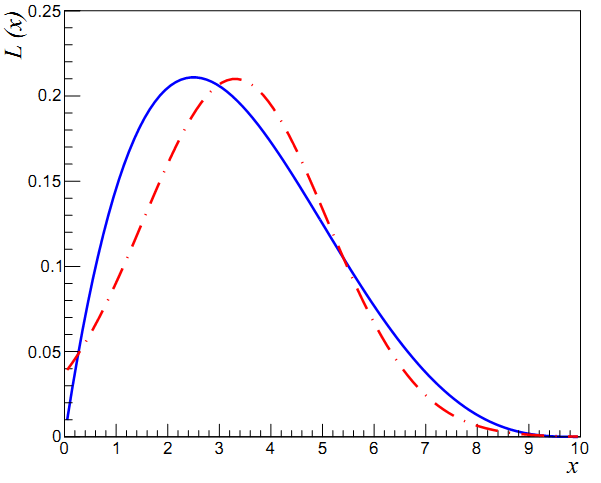
\includegraphics[width=7.cm]{veri_l1}}
\vspace{-0.2cm}
\caption{Fun\c{c}\~{a}o de verossimilhan\c{c}a (linha cont\'{\i}nua) para uma amostra de um sucesso em 4 tentativas  de extra\c{c}\~{a}o de bolas azuis de uma caixa contendo  10 bolas. A linha pontilhada \'{e} uma distribui\c{c}\~{a}o  gaussiana de mesmo valor esperado e desvio padr\~{a}o da fun\c{c}\~{a}o de verossimilhan\c{c}a normalizada.}
\label{azul_vero_fig}
\end{figure}


%

Ao se obter tr\^{e}s amostras  de quatro tentativas de extra\c{c}\~{a}o de bolas azuis, por exemplo, duas amostras de um sucesso ($m=1$) e uma de dois sucessos ($m=2$), a  fun\c{c}\~{a}o de verossimilhan\c ca \'e dada por (Fig.~\ref{verossimil})
   $${\cal L} (x) \ \propto \ B (1|4; x/10)^2 \times  B (2|4; x/10)$$
o que implica, igualmente, o valor 3 como a melhor estimativa para a quantidade de bolas azuis.
\begin{figure}[hbtp]
\centerline{\includegraphics[width=7.cm]{veri_l2}}
\vspace{-0.2cm}
\caption{Fun\c{c}\~{a}o de verossimilhan\c{c}a (linha cont\'{\i}nua)  para 2 amostras de um sucesso, e uma de dois sucessos em 4 tentativas de extra\c{c}\~{a}o  de bolas azuis de uma caixa contendo 10 bolas. A linha  pontilhada \'{e} uma gaussiana de mesmo valor esperado e desvio padr\~{a}o.}
\label{verossimil}
\end{figure}



%%%%%%%%%%%%%%%%%%%%%%%%%%%%%%%%%%%%%%%%%%%%%%%%%%%%%%%%%%%%%%%%%
%\pagebreak
Desse modo,  Fisher considera que o \index{estimadores! de m\'{a}xima verossimilhan\c{c}a}\index{maxima@m\'{a}xima verossimilhan\c{c}a! estimadores de}{\bf estimador  de m\'{a}xima verossimilhan\c{c}a}\footnote{Maximum likelihood estimator.} ($\hat \theta$)  para o  par\^{a}metro $\theta$ \'{e} aquele que maximiza a  fun\c{c}\~{a}o de verossimilhan\c{c}a, ou seja,
\begin{equation}
 \label{cond_vero}
\left. \frac{\partial {\cal L}}{\partial \theta}\right|_{\hat \theta} = 0
 \end{equation}

Uma vez que o logaritmo de ${\cal L}$ atinge seu m\'{a}ximo para o mesmo valor de $\theta$ e ${\cal L}$, a condi\c{c}\~{a}o de m\'{a}xima verossimilhan\c{c}a \'{e} expressa como
\begin{equation}
 \label{cond_vero2}
\left.  \frac{\partial \ln {\cal L}}{\partial \theta}\right|_{\hat \theta} = 0
 \end{equation}
ou seja, o estimador de m\'{a}xima verossimilhan\c{c}a \'{e} raiz da equa\c{c}\~{a}o anterior (Eq.~\ref{cond_vero2}).



%%%%%%%%%%%%%%%%%%%%%%%%%%%%%%%%%%%%%%%%%%%%%%%%%%%%%%%%%%%%%%%%%

%Para 30 amostras (Fig.~\ref{verossimil2}) de um sucesso (uma bola azul) e uma de dois sucessos (duas bolas azuis),obt\'{e}m-se
%   $${\cal L}^{31} (x) = B (1,4,x/10)^{30} \times  B (2,4,x/10)$$

%\begin{figure}[hbtp]
%\centerline{\includegraphics[width=8cm]{Fig/veri_l2}}
%\caption{Fun\c{c}\~{a}o de verossimilhan\c{c}a para 30 amostras de um sucesso, e uma de dois sucessos de extra\c{c}\~{a}o  e bolas azuis. A linha pontilhada \'{e} uma distribui\c{c}\~{a}o  gaussiana de mesma m\'edia e vari\^ancia.}
%\label{verossimil2}
%\end{figure}


\pagebreak
  Mesmo que o dom\'{\i}nio da vari\'{a}vel aleat\'{o}ria $x$ seja cont\'{\i}nuo, como usualmente as medidas de uma grandeza, as amostras constituem sequ\^{e}ncias discretas de valores organizados em $M$ classes de intervalos $\Delta_i$, como
$$ \Big\{ (x_1, x_2 = x_1 + \Delta_1) ;  (x_2, x_3 = x_2 + \Delta_2) ;  \dots  ; (x_M, x_{M+1} = x_M + \Delta_M) \Big\}$$


 Nesse caso, a probabilidade associada a essa sequ\^{e}ncia particular  \'{e}  dada por
%$$  \prod_{i=1}^{N} \int_{x_i}^{x_i + \Delta_i} \rho(x_i|\theta) \, \mbox{d}x_i $$
$$  \int_{x_1}^{x_2} \int_{x_2}^{x_3} \! \ldots  \int_{x_M}^{x_{M + 1}} \rho(x_1|\theta) \rho(x_2|\theta) \ldots \rho(x_M|\theta) \ \mbox{d}x_1 \, \mbox{d}x_2  \ldots \, \mbox{d}x_M $$

% Se os intervalos $\Delta_i$ s\~{a}o ``suficientemente pequenos'', pode-se escrever
%$$  \bigg( \underbrace{\prod_{j=1}^{N} \Delta_j}_{K = \, \mbox{\tiny cte.}} \bigg)  \prod_{i=1}^{N} \rho(x_i|\theta) $$
 e define-se a fun\c{c}\~{a}o de verossimilhan\c{c}a por
\begin{equation}
 \label{vero2}
\fbox{~$\displaystyle  {\cal L} (x_1, x_2, x_3 \dots  x_M; \theta)  = K \ \prod_{i=1}^{M} \rho(x_i|\theta)
$~}
 \end{equation}
em que $K$ \'{e} uma constante arbitr\'{a}ria.
\newpage
\section{Exerc\'{\i}cios}
\label{exerc_likeli}

\begin{itemize}

\item[\ref{exerc_likeli}.1)]
Ao colidir com a superf\'{\i}cie terrestre, um meteoro provoca uma cratera. A rela\c{c}\~{a}o esperada entre o di\^{a}metro ($D$) da cratera e a energia cin\'{e}tica ($E$) do meteoro no instante do impacto \'{e} dada por
$$ D = k E^{1/4} $$
em que $k$ \'{e} uma constante.

A tabela abaixo mostra os di\^{a}metros das depress\~{o}es causadas pelo impacto de diversas esferas de a\c{c}o sobre a areia contida em uma caixa, e as correspondentes  incertezas ($\epsilon_D$) e energias cin\'{e}ticas das esferas ao colidirem com a areia da caixa. As esferas s\~{a}o utilizadas para simularem a queda de meteoros.

\renewcommand{\arraystretch}{1.14}

%\vspace{0.1cm}

\hspace{0.3cm}
\begin{center}
{\small
\begin{tabular}{c|c|c}
        $E$(J)  &  $D$(cm)  &  $\epsilon_D$(cm) \\ \hline
     0,07 &   4,9 &  0,3  \\
     0,18 &   6,7 &  0,3  \\
     0,30 &    7,3 &   0,4  \\
     0,45  &   8,1  &  0,4   \\
     0,69 &    9,2 &   0,4  \\
  \hline
      \end{tabular}
}
\end{center}
\renewcommand{\arraystretch}{1}



\vspace{0.5cm}
A partir de um ajuste linear, determine uma estimativa para o expoente da rela\c{c}\~{a}o esperada entre a energia e o di\^{a}metro.

%\bibliographystyle{plainnat}
%\bibliography{biblio}


\end{itemize}

